\documentclass[a4paper]{article}

%====================== PACKAGES ======================

\usepackage[utf8x]{inputenc}
\usepackage[french]{babel}
\usepackage{graphicx}
\usepackage{hyperref}
\usepackage{array}
\usepackage{tabularx}
\usepackage{setspace}
\usepackage[T1]{fontenc}
\usepackage[top=2.5cm, bottom=2.5cm, left=2.5cm, right=2.5cm]{geometry}
\usepackage{fancyhdr}
\usepackage{wrapfig}
\usepackage{filecontents}
\usepackage{tikzsymbols}

%====================== INFORMATION ET REGLES ======================

%rajouter les numérotation pour les \paragraphe et \subparagraphe
\setcounter{secnumdepth}{4}
\setcounter{tocdepth}{4}

\hypersetup{
pdfauthor = {Julien Schoumacher},
pdftitle = {Stage de fin d'étude -
           Etude de sécurité d'un contrôleur SDN : ONOS},
pdfsubject = {Mémoire de stage d'ingénieur},
pdfkeywords = {SDN, ONOS, sécurité},
pdfstartview = {FitH}}

\graphicspath{ {images/} }


%====================== Bibliographie ======================
\begin{filecontents}{references.bib}
@online{indirection,
  title = {Niveau d'indirection supplémentaire},
  url = {https://en.wikipedia.org/wiki/Fundamental_theorem_of_software_engineering},
}
\end{filecontents}

\begin{filecontents}{references.bib}
@online{rapport_maxence,
  title = {Mémoire de stage : Étude d’OpenFlow dans le contexte de la sécurité},
  author = {Maxence Tury}
}
\end{filecontents}

\begin{filecontents}{references.bib}
@online{histoire,
  title = {A Survey of Software-De ned Networking:  Past,
Present, and Future of Programmable Networks},
  author = {Bruno Nunes Astuto, Marc Mendonça, Xuan Nam Nguyen, Katia Obraczka,Thierry Turletti}
  url = {https://hal.inria.fr/hal-00825087/file/hal_final.pdf}
}
\end{filecontents}

\begin{filecontents}{references.bib}
@online{OF_10,
  title = {Spécification Openflow 1.0},
  url = {http://archive.openflow.org/documents/openflow-spec-v1.0.0.pdf}
}
\end{filecontents}

\begin{filecontents}{references.bib}
@online{OF_15,
  title = {Spécification Openflow 1.5},
  url = {https://www.opennetworking.org/images/stories/downloads/sdn-resources/onf-specifications/openflow/openflow-switch-v1.5.0.noipr.pdf}
}
\end{filecontents}


%======================== DEBUT DU DOCUMENT ========================
\newgeometry{top=3.5cm}
\pagestyle{fancy}
\fancyhf{}
\fancyhead[C]{~\\}
\fancyfoot[C]{\thepage}

\begin{document}

%régler l'espacement entre les lignes
\newcommand{\HRule}{\rule{\linewidth}{0.5mm}}

%page de garde
\begin{titlepage}
	\newcolumntype{s}{>{\hsize=.25\hsize}X}
	\begin{tabularx}{\textwidth}{lsrl}
		
\includegraphics[width=0.2\textwidth]{TelecomParisTech_logo_200_01.png}
		&
    	\shortstack{\huge{Télécom} \\ \huge{ParisTech}}
    	&
		
\includegraphics[width=0.2\textwidth]{Logo_SP.jpg}
		&
		\shortstack{\huge{Télécom} \\ \huge{SudParis}}
	\end{tabularx}

    \begin{center}
        \vspace*{1cm}
        
        \Huge
       	~\\
       	~\\
       	~\\
        \textbf{Mémoire de stage}
        
        \vspace{0.5cm}
        \LARGE
        Sécurité d'un contrôleur SDN : ONOS\\
        ~\\
        
        \vspace{1.5cm}
        
        \textbf{Julien Schoumacher}
        
        \vfill
       
        \begin{flushleft}
       		 Diplôme préparé : Ingénieur\\
        	 Stage effectué du 20 juillet 2016 au 20 janvier 2017 à Télécom SudParis sous la direction de Grégory Blanc
        \end{flushleft}
        \vspace{0.3cm}
        
    \end{center}
\end{titlepage}

%======================== Remerciements ========================
\newpage
~
\section*{\Huge{Remerciements\\}}
\Large Avant d'entamer la lecture de ce rapport, je tiens avant tout à remercier toute l'équipe du département RST (Réseaux et Services des Télécommunications) de Télécom SudParis qui m'a si bien accueilli durant ce stage. Je remercie également mon encadrant côté Télécom ParisTech Rida Khatoun, m'ayant mis en relation avec le maître de conférences Gregory Blanc qui m'a encadré avec bienveillance pendant toute la durée du stage. Enfin, toutes les autres personnes que j'ai pu cottoyer plus ou moins longtemps à l'occasion d'évènements ponctuels comme la conférence RAID qui s'est tenue en septembre.
\phantomsection


%======================== Table des matières ========================
\newpage
\tableofcontents


\newpage
\fancyhead[L]{1- Réseau SDN}
\section{Réseau SDN (Software Defined Network)}
	\subsection{Motivation}
		On ne peut pas entamer cette étude portant en partie sur les réseaux SDN sans oublier de mentionner quelques éléments difficilement contestables sur les réseaux actuels \footnote{\label{of_def}Aussi résumé dans \url{https://www.opennetworking.org/sdn-resources/sdn-definition}} :

\begin{itemize}

\item La demande ne cesse de croître : on observe un accroissement considérable des enjeux liés au traitement de masse importante de données, de l'utilisation de services cloud, du trafic mobile et peut être bientôt de l'utilisation d'objets connectés. Or tous ces éléments présentent le point commun de communiquer avec de nombreuses entités situées sur des réseaux potentiellement éloignés. Cela mobilise donc un trafic réseau intense.

\item Les technologies actuelles pour soutenir cette demande énorme sont capables de fournir un débit titanesque : que l'on considère des technologies sans fil ou non, au coeur des réseaux tant au niveau des terminaux des utilisateurs, on atteint aujourd'hui des débits théoriques de l'ordre du Gigabit par seconde pour l'utilisateur. Tout cela sans que l'on ait vraiment conscience des conditions que cela requiert.

\item Les méthodes d'accès sont aujourd'hui bien différentes. Précédemment le modèle client/ serveur était largement employé, avec dans le cas d'une entreprise, un réseau interne constitué de plusieurs LAN séparés, et connecté à internet de manière quasiment unique. Cela entraînant une configuration possiblement statique et donc aisée, les échanges se déroulant principalement sur un mode requête/réponse. Or la tendance, notamment à cause des deux premiers points, est à l'émergence de nouveaux modes d'accès plus horizontaux (avec d'avantage d'entités faisant circuler l'information au même niveau "hiérarchique"). Ce type de communication tient entre autres de la distribution plus éparse des données à travers le réseau due au grossissement de la taille des bases de données, à la duplication de celles-ci (mise en cache sur différents serveur à travers le monde pour permettre un accès plus rapide), à l'augmentation du trafic volumineux (vidéo, voix) et de nouveaux trafics (IoT, Bring Your Own Device, ...) même au sein de l'entreprise. Enfin, l'utilisation de plus en plus répandue de services cloud, avec ses implications au niveau de la virtualisation (que ce soit des applications, ou bien des bases de données), susceptible de changer en permanence la localisation des serveurs pour garantir une certaine flexibilité.

\end{itemize}

Or, le réseau principal global tel que nous le connaissons (la partie reposant sur TCP/IP en tout cas) a été conçu d'abord dans un but de fiabilité : chaque paquet doit être reçu, peu importe la route empruntée. L'architecture distribuée actuelle n'est donc pas bâtie pour assurer spécifiquement une extension aisée des services fournis, ni une qualité de service définie. Le routeur (et le réseau d'ailleurs) des années 1980 a donc été progressivement amélioré sur la base de ce paradigme initial, avec le plan de données et le plan de contrôle attachés aux mêmes équipements, configurés en partie manuellement. Tout s'est complexifié également : nouveaux protocoles, ajouts d'équipements spécifiques (capables de répartir la charge réseau, de filtrer les paquets, de prévenir de certaines tentatives d'attaque, etc ...), ...\\
Certains éléments de réflexion peuvent éventuellement nous mettre sur la voie d'une complexité qui, à défaut d'être exponentielle, l'est d'avantage que simplement linéaire (c'est du moins une conviction personnelle non vérifiée) :

\begin{itemize}
\item Plus il y a d'éléments statiques dans un réseau, et plus la propagation des modifications d'ensemble est coûteuse (puisqu'il faut penser à chaque impact sur les parties statiques et modifier un à un chaque équipement).
\item Si un problème survient, il est difficile d'avoir une vue globale de ce qui se passe puisqu'à moins de disposer d'équipements spéciaux aucune vue globale du réseau n'est accessible : il faut vérifier (potentiellement) que chaque élément se comporte correctement et est bien configuré.
\item Les interfaces entre switchs, routeurs et autres éléments peuvent varier selon le constructeur, et le logiciel sur les équipements est souvent propriétaire et complexe, surtout dans le cas de gros réseaux hétérogènes, ce qui ne facilite pas forcément la bonne marche de l'ensemble.
\end{itemize}

De nombreux problèmes se résolvent avec un niveau d'abstraction supplémentaire \footnote{\label{indirection}\url{https://en.wikipedia.org/wiki/Fundamental_theorem_of_software_engineering}}. Si le dévelop-pement de systèmes de plus en plus complexes s'est fait de manière très rapide sur PC, c'est d'abord grâce à la première couche d'abstraction qu'ont constitué les instructions assembleur, puis à la seconde qu'a été le système d'exploitation. Certaines personnes ont eu l'idée, au lieu de considérer le réseau comme un élément périphérique, de le voir comme un processeur capable d'exécuter des instructions basiques, fournissant de fait un service plus facilement adaptable. C'est sur ce principe que repose le Software Defined Network (SDN). Avec une couche d'abstraction supplémentaire que constitue le protocole choisi pour véhiculer le flot d'instructions (OpenFlow dans notre cas, mais il y en a d'autres que nous évoquerons succintement plus tard), et un système d'exploitation spécifique (Network Operating System, NOS), l'idée est de découpler les différents chemins qu'empruntent les données et le plan de contrôle, à la manière d'un système d'exploitation qui sépare le code d'un programme et les données qu'il utilise.
		~\\
	\subsection{Concepts}
		La dernière analogie (avec un ordinateur) peut être poursuivie de la manière suivante. Sur un PC classique, on crée et utilise des applications qui reposent sur un système d'exploitation responsable des éléments matériels. De manière similaire, le modèle SDN permet la création d'applications "réseau" sans se soucier de la traduction des décisions de routage des paquets au niveau applicatif en routage au niveau des interfaces physiques.\\

Pour réaliser cela, il est nécessaire, puisqu'un réseau est constitué d'entités physiquement séparées, de disposer d'un protocole de communication standard entre celles-ci. Mais ça n'est pas suffisant : des instructions de routage doivent également être distribuées. Cela n'est possible que si il existe un cerveau central qui coordonne les opérations (il n'existe pas vraiment d'intelligence collective à ce jour). C'est le rôle du contrôleur SDN. On déporte ainsi l'intelligence humaine déployée dans la configuration de tous les éléments du réseau vers un seul (même si il peut être dupliqué).\\

\begin{figure}[h]
  	\centering
  	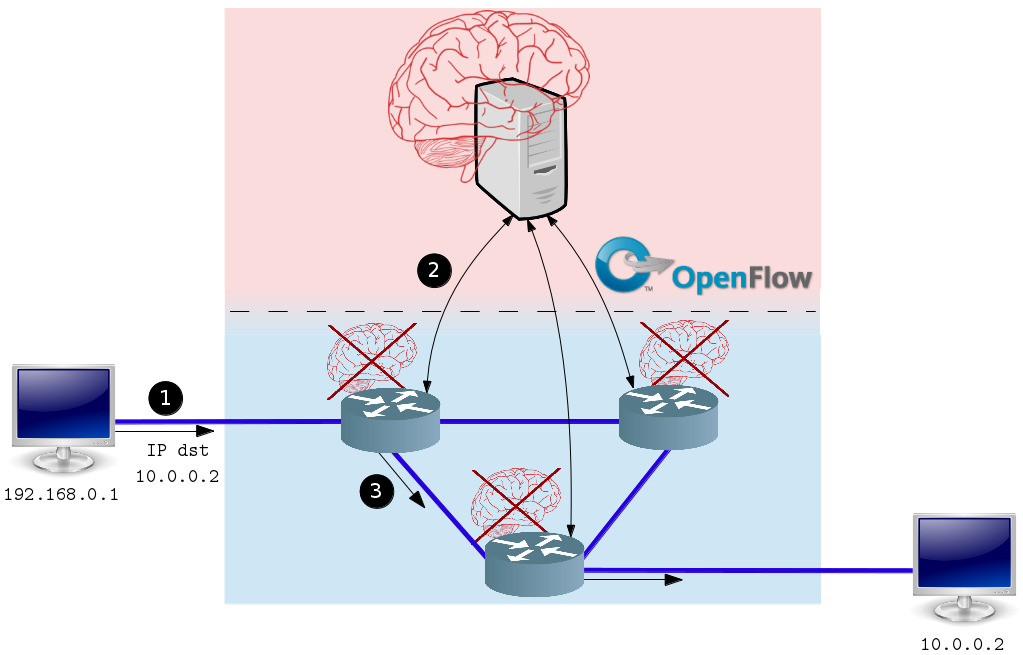
\includegraphics[width=0.8\textwidth]{openflow.png}
  	\caption[Caption for LOF]{Réseau SDN : "l'intelligence" est déportée vers le contôleur \footnotemark}
\end{figure}

\footnotetext{\label{rapport_maxence} Schéma extrait du mémoire "Étude d’OpenFlow dans le contexte de la sécurité" de Maxence Tury}

\begin{figure}[h]
  	\centering
  	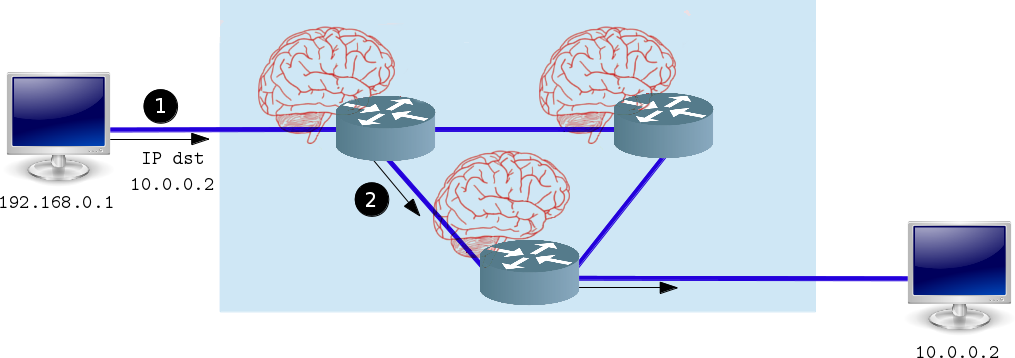
\includegraphics[width=0.85\textwidth]{routage_normal.png}
  	\caption{Réseau classique : chaque routeur contient une partie de la logique de contrôle}
\end{figure}

Les avantages de cette architecture sont multiples :
\begin{itemize}
\item D'abord cela réduit grandement la complexité de configuration manuelle et le risque d'erreur (si le système d'exploitation réseau est fiable).
\item Cela facilite donc énormément le développement d'applications réseau complexes, puisque la tâche peut être quasiment séparée de sa réalisation physique.
\item Les routes optimales sont plus facilement calculables qu'au sein d'un réseau classique : un seul élément gère les différentes distances et métriques qui peuvent changer selon le trafic, et être modifiées à la volée par des applications spécifiques.
\item La gestion du réseau devient plus simple, les évènements importants (perte d'un lien, dysfonctionnement, ralentissement ...) peuvent être remarqués rapidement, la réaction pouvant être automatique et quasiment instantanée.
\item Les coûts matériels sont globalement diminués puisqu'un switch programmable Openflow peut n'implémenter que le protocole en question pour être fonctionnel (le reste pouvant être pris en charge logiciellement au niveau du contrôleur). Il est également possible de migrer partiellement vers une architecture SDN en utilisant des switchs hybrides.
\end{itemize}

Pour résumer, beaucoup plus de flexibilité est permise par cette approche, économisant temps et matériel. Évidemment, l'idée n'est pas nouvelle, mais n'a pas que des avantages. Notamment : la sécurité du contrôleur devient un point brûlant, puisque toute la gestion du réseau repose sur lui.
		~\\
	\subsection{Historique}
		L'idée d'une séparation entre plan de données et plan de contrôle n'est pas nouvelle, et cette partie se propose de retracer succinctement diverses voies qui ont abouti à l'adoption assez univoque du protocole OpenFlow comme interface entre les deux. Pour obtenir un état de l'art détaillé et complet, il est possible de consulter les articles "A Survey of Software-Defined Networking: Past, Present, and Future of Programmable Networks"\footnote{\label{histoire}\url{https://hal.inria.fr/hal-00825087/file/hal_final.pdf}} (2014) et "Software-Defined Networking: A Comprehensive Survey"\footnote{\url{http://www.hit.bme.hu/~jakab/edu/litr/SDN/Long_Survey_06994333.pdf}} (2015).\\

Assez tôt est apparue l'idée de rendre les switchs programmables : dès 1990, le groupe Open Signaling propose un protocole de contrôle de switchs à distance appelé GSMP (General Switch
Management  Protocol). Si les possibilités restent assez limitées (essentiellement gestion des ports, redirection de trafic sur des ports contrôlés, et obtention de statistiques), cela permet néanmoins un accès au matériel plus aisé.

D'autres approches sont testées dans la même période : l'initiative Active Networking propose quant à elle un mécanisme de propagation de code que l'équipement réseau exécute lorsqu'il reçoit les paquets encapsulant le code (même si cela pose un gros problème en matière de sécurité).

Le groupe DCAN (Devolved Control of ATM Networks) propose une approche qui se rapproche très fortement du paradigme SDN : ils développent un protocole minimaliste entre une entité spécialisée (le contrôleur) et autres équipements et mettent en place une gestion semi-automatique du réseau pour partitionner les ressources disponibles (ils rajoutent donc la possibilité de programmer le contrôleur).\\

Le projet 4D \footnote{\url{http://www.cs.cmu.edu/~4D/}} initié en 2004, présente une formalisation du concept : on cherche à obtenir la possibilité de prendre des décisions réseau en dehors des équipements physiques, ce qui nécessite l'obtention d'un maximum d'informations à la fois sur la composition physique du réseau, et sur les liens qui existent entre chaque élément. L'incorporation des services globaux que sont la découverte de la topologie et la dissémination d'informations sur l'état général du réseau associée à la possibilité d'agir sur le réseau est ce qui a inspiré l'idée de système d'exploitation réseau, qu'implémentent aujourd'hui les contrôleurs SDN.\\

On peut encore citer NETCONF et Ethane (2006), le premier pouvant être vu comme une extension de SNMP, le second comme un ancêtre immédiat d'OpenFlow. Même si la finalité d'Ethane était plus axée sur une gestion des identités (vérification des droits d'un paquet à circuler sur le réseau entre autres) que sur une gestion générale du réseau, c'est un protocole entre switch programmable et contrôleur encapsulant des actions à effectuer sur des paquets reçus au niveau du switch (ces actions étant essentiellement limitées à de la redirection/suppression).\\

OpenFlow a quant à lui précédé l'apparition du terme SDN lors d'expérimentations à Stanford vers 2010 (la première spécification d'OpenFlow pour la production (1.0.0), a été publiée début 2010).
		~\\
	\subsection{Exemples d'applications}
\section{Cadre de l'étude}
	\subsection{Problématique et objectifs}
	\subsection{Architecture d'un réseau SDN}
		\subsubsection{Openflow}
		\subsubsection{Contrôleur SDN}
		\subsubsection{ONOS}
	\subsection{Surface d'attaque}
		\subsubsection{Menaces au niveau de l'interaction avec les switchs}
		\subsubsection{Menaces au niveau de l'interaction utilisateur}
		\subsubsection{Autres menaces}
	\subsection{Scénarios envisagés}
\section{Audit}
	\subsection{Man in the middle au niveau de l'interface sud}
	\subsection{Altération de la topologie depuis l'interface sud}
	\subsection{Deni de service au niveau de l'interface sud}
	\subsection{Deni de service au niveau de l'interface nord}
	\subsection{Fuites d'information au niveau de l'interface nord}
	\subsection{Mauvaise configuration au niveau de l'interface nord}
\section{Validation et évaluation}
	\subsection{Résultats de l'étude}
	\subsection{Autres considérations}
\section{Perspectives à l'issue du stage}
\section{Ressources}


~

\newpage

%récupérer les citation avec "/footnotemark"
\nocite{*}

%choix du style de la biblio
\bibliographystyle{plain}
%inclusion de la biblio
\bibliography{bibliographie.bib}
%voir wiki pour plus d'information sur la syntaxe des entrées d'une bibliographie

\end{document}
